\documentclass[11pt]{article}%

\usepackage{styles/style}

\begin{document}
\section{Contraction ratio with uncertainty}
\[\frac{x'_{l}}{x} = \frac{f_{-}(x, \theta)}{x} = \frac{\sin(\theta + \delta)}{\sin(\theta + \delta - \phi)} \eqqcolon a\]
\[\frac{y'_{u}}{y} = \frac{f_{+}(y, \theta)}{y} = \frac{\sin(\theta - \delta)}{\sin(\theta - \delta - \phi)} \eqqcolon b\]
\[UC(\theta, \phi) = \frac{y'_u- x'_l}{y-x} = \frac{by-ax}{y-x} = b+(b-a)\frac{x}{y-x}\]

Since $b > a$, if $y-x$ remains the same, then as $x$ increases, the contraction ratio with uncertainty increases; if $x$ remains the same, then as $y$ increases, the contraction ratio with uncertainty decreases.

\begin{figure}[!h]
  \centering
  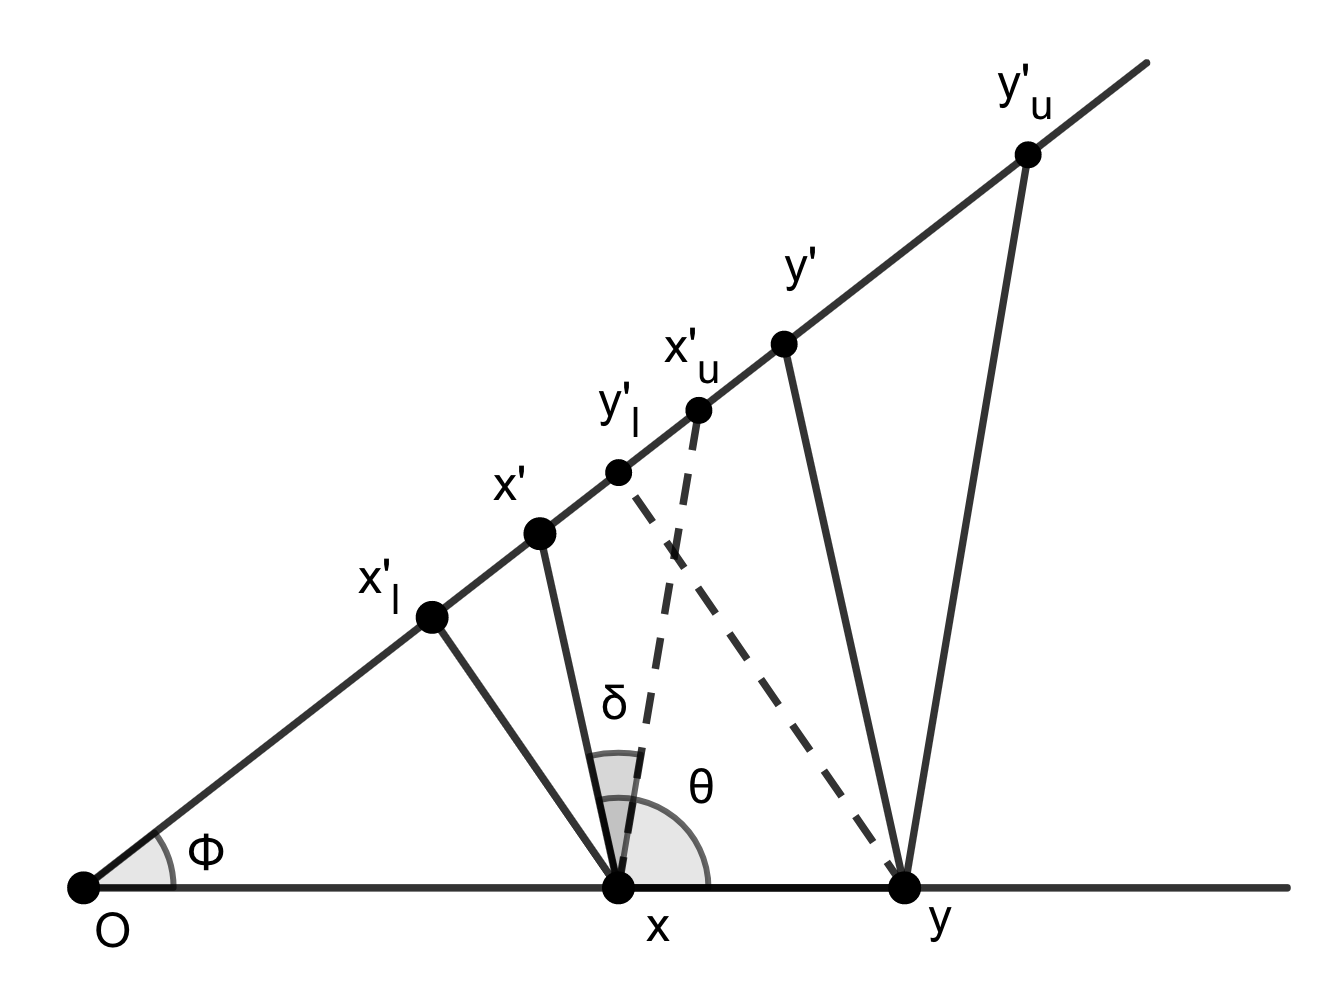
\includegraphics[width=0.7\linewidth]{uncertainty_bounce.png}
  \caption{Bounce with uncertainty}
  \label{fig:uncertain_bounce}
\end{figure}
\end{document}